% Nama Kelompok : Kelompok 3
% Kelas : D4 TI 1A
% 1. Kadek Diva Krishna Murti (1174006)
% 2. Niko Eklesia
% 3. Rizal Rony Sitorus
% 4. Jeremia Wahyudi Sianturi (1174029)
% 5. Sri Rahayu (1174015)

\section{Sejarah Bit Parity}
Sebuah "paritas track" hadir pada penyimpanan data pita magnetik pertama pada tahun 1951. Paritas dalam bentuk ini, diterapkan di beberapa sinyal paralel, dikenal sebagai cek redundansi transversal. Ini dapat dikombinasikan dengan paritas yang dikomputasi melalui beberapa bit yang dikirim pada sinyal tunggal, pemeriksaan redundansi longitudinal. Dalam bus paralel, ada satu bit cek redundansi longitudinal per sinyal paralel. Paritas juga digunakan setidaknya pada beberapa sistem pemasukan pita kertas (tape berlubang) (yang mendahului sistem pita magnetik). Pada sistem yang dijual oleh perusahaan Inggris ICL (sebelumnya ICT), pita kertas berukuran 1 inci (25 mm) memiliki 8 posisi lubang yang melintang di atasnya, dengan posisi ke 8 untuk paritas. 7 posisi digunakan untuk data, misalnya, 7-bit ASCII. Posisi 8 memiliki lubang yang dilubangi tergantung pada jumlah lubang data yang dilubangi.


\section{Pengertian Bit Parity}
Bit Parity merupakan bit tambahan yang disisipkan pada urutan bit-bit data yang ditransmisikan. Adapun tujuan dari pemberian bit parity ini yaitu untuk memastikan bit - bit yang ditransmisikan tidak mengalami perubahan nilai setelah sampai ke penerima. Perubahan nilai tersebut dapat terjadi karena pengaruh noise atau sinyal liar.
Perubahan nilai tersebut, seperti 0 $\,\to\,$ 1 atau 1 $\,\to\,$ 0

Contoh :

\begin{table}[h!]
\centering
\begin{tabular}{ c c c }
0110100 & $\,\to\,$ &  0100100\\
\hline
Tx &  & Rx \\
\end{tabular}
\end{table}

\begin{figure}[ht]
\centerline{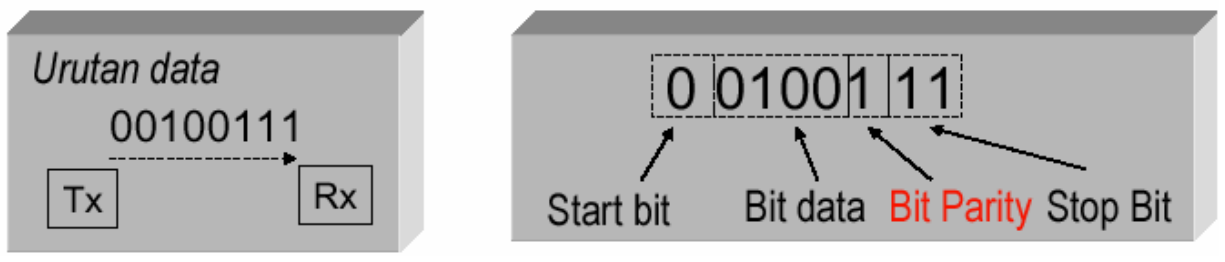
\includegraphics[width=1\textwidth]{figures/perubahan_nilai_bit_parity.png}}
\caption{Contoh perubahan nilai pada bit parity.}
\label{perubahan_nilai_bit_parity}
\end{figure}

Proses perubahan nilainya bisa dilihat pada gambar \ref{perubahan_nilai_bit_parity}

Parity-bit diperoleh dengan menghitung satuan data yang akan dikirim sehingga dengan menghitung kembali parity-bit pihak penerima data dapat memperkirakan data yang diterima rusak atau tidak.

\section{Jenis - Jenis Bit Parity}
Berdasarkan jurnal yang berjudul “Perangkat Komunikasi Multi - External Hardware Melalui LAN Dengan Menggunakan Microcontroller” oleh Marojahan M.T. Sigiro \cite{sigiro2013perangkat} menyatakan terdapat beberapa macam parity yang ada dalam proses pengiriman data, yaitu sebagai berikut : 
\begin{enumerate}
\item Even parity, bernilai 0 jika bit 1 yang dikirim berjumlah genap dan bernilai 1 jika bit 1 yang dikirim berjumlah ganjil. 
\item Odd parity, bernilai 0 jika bit 1 yang dikirim berjumlah ganjil dan bernilai 1 jika bit 1 yang dikirim berjumlah genap. 
\item Mark parity 
\item Space parity
\end{enumerate}

Contoh :
\newline Berikan tambahan Even Parity bit pada urutan data berikut ini :
\newline Jawab :
\begin{verbatim}
1001		-> 0
00111101	-> 1
10110		-> 1
\end{verbatim}

Tabel Kebenaran

Odd Parity Bit yang dibangkitkan dari urutan data 3 bit biner (ABC)
\begin{table}[h!]
\begin{tabular}{|c|c|c|c|}
\hline
\multicolumn{3}{|c|}{Input} & Output\\
\hline
A & B & C & P\\
\hline
0 & 0 & 0 & 1\\
\hline
0 & 0 & 1 & 0\\
\hline
0 & 1 & 0 & 0\\
\hline
0 & 1 & 1 & 1\\
\hline
1 & 0 & 0 & 0\\
\hline
1 & 0 & 1 & 1\\
\hline
1 & 1 & 0 & 1\\
\hline
1 & 1 & 1 & 0\\
\hline
\end{tabular}
\end{table}

Even Parity Bit yang dibangkitkan dari urutan data 3 bit biner (ABC)
\begin{table}[h!]
\begin{tabular}{|c|c|c|c|}
\hline
\multicolumn{3}{|c|}{Input} & Output\\
\hline
A & B & C & P\\
\hline
0 & 0 & 0 & 0\\
\hline
0 & 0 & 1 & 1\\
\hline
0 & 1 & 0 & 1\\
\hline
0 & 1 & 1 & 0\\
\hline
1 & 0 & 0 & 1\\
\hline
1 & 0 & 1 & 0\\
\hline
1 & 1 & 0 & 0\\
\hline
1 & 1 & 1 & 1\\
\hline
\end{tabular}
\end{table}

\subsubsection{Parity Generator}

Parity generator merupakan sebuah rangkaian untuk membangkitkan atau membuat bit parity. Bit Parity dibangkitkan dari urutan data yang terdiri dari sejumlah bit biner. Bit Parity dibuat sebelum data ditransmisikan, karena itu Parity Generator letaknya di Transmitter.

\subsubsection{Parity Checker}

Parity checker merupakan sebuah rangkaian untuk mengecek urutan bit - bit data dan bit parity (yang telah dibangkitkan oleh Parity Generator) setelah ditransmisikan. Parity Checker menghasilkan nilai "0" atau "1" yang menunjukkan indikasi kesalahan bit saat diterima. Apabila Nilai Indikator Kesalahan adalah "1" maka bit yang diterima salah, dan apabila "0" maka bit-bit yang diterima benar. Parity checker berada di sisi receiver.

\section{Cara Kerja Bit Parity}
\subsection{Konsep Umum}
Pihak pengirim akan menambahkan 1 bit tambahan (Bit Parity) pada data, untuk menggabarkan karakteristik dari data tersebut. Nilai dari bit parity (1 atau 0) tidak diperbolehkan secara sembarang. Dalam proses pentransmisiannya data tadi dikirim bersamaan (data dan bit parity-nya). Pada terminal penerimaan data kita dibaca dan di dekodisasi dengan cara yang sama seperti saat menentukan nilai bit parity disisi pengirim. Lalu hasil dekodisasi tersebut dibandingkan dengan bit - bit parity yang dikirim oleh pengirim. Apabila hasil pembacaan (dekodisasi) data terkirim sama dengan bit paritynya maka data tersebut dapat dianggap benar dan apabila diperoleh perbedaan nilai antara hasil dekodisasi dengan bit paritynya maka data dapat diklasifikasi sebagai data yang error. Terminal penerima akan mengirim permintaa pada terminal pengirim untuk mengirim ulang data yang error.
 
\subsection{Menentukan Nilai Bit Parity}
Penentuan nilai bit Parity (1 atau 0) dilakukan dengan meng-XOR kan semua bit yang ada pada data sepasang-sepasang, hasil akhir dari peng-XOR an seluruh bit ini yang akan dijadikan acuan untuk menentukan nilai dari bit Parity yang akan ditambahkan. Jadi belum tentu hasil XOR langsung dijadikan sebagai nilai dari bit Parity. Contohnya dapat dilihat pada gambar \ref{ilustrasixorgate}

\begin{figure}[ht]
\centerline{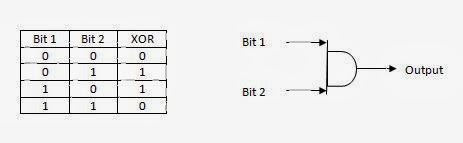
\includegraphics[width=1\textwidth]{figures/ilustrasixorgate.jpg}}
\caption{Kiri = Tabel XOR ; Kanan = ilustrasi XOR Gate}
\label{ilustrasixorgate}
\end{figure}

Misal data yang berupa 1 karakter adalah huruf  "M", yang menurut ASCII sama dengan 1011001, maka proses XOR nya =\\
1 XOR 0 = 1\\
1 XOR 1 = 0\\
0 XOR 1 = 1\\
1 XOR 0 = 1\\
1 XOR 0 = 1\\
1 XOR 1 = 0\\
Jika bit 1 pada data berjumlah ganjil maka keluaran akhirnya adalah "1", dan jika genap maka keluaran akhirnya adalah "0". 

%%%%%%%

\subsection{Skema XOR}
Bit 0 adalah bit pertama begitu seterusnya. Setelah kita hasil dari XOR barulah kita akan menentukan nilai dari bit Parity data kita. Ada bit Parity ganjil dan Parity genap, Parity genap maka hasi XOR itu adalah nilai bit Parity, jika Parity ganjil maka nilai bit Parity merupakan nilai komplement (kebalikan) dari hasil XOR.

\subsection{Contoh Cara kerja Bit Party}
Ada 2 orang sedang melakukan chatting, keduanya melakukan percakapan. Metode Pendeteksi Error menggunakan Bit Parity.\\
Orang pertama mengirim kata "Aku" ke orang kedua.\\
Dalam kode ASCII berarti =\\
A = 1000001\\
k = 1101011\\
u = 1010111\\
Dalam terminal pengirim kata "Aku" dianalisa perkarakter "A" lalu "k" lalu "u"  dari masing masing huruf diberikan bit Paritynya (menggunakan Even Parity bit/ Parity Genap) . Maka data akan berubah menjadi :\\
A = 10000010\\
k = 11010111\\
u = 10101111\\
Data lalu dikirim dengan format: 10101111\_11010111\_10000010\\
Karena terjadi suatu hal seperti distorsi atau noise-noise lainnya, bit-bit tadi ada yang berubah dalam perjalannya menjadi :\\
10101111\_11010111\_11000010\\
Pada sis penerima data tersebut terbaca "Cku" bukan "Aku", bila tanpa metode deteksi Error maka data tersebut dianggap valid dan penerima mendapat kesusahan dalam membacanya.\\ \\
Mekanisme Pembacaannya :
\begin{itemize}
\item Bit 1100001 didekondisasikan dan akan menghasilkan bit "1"
\item Penerima membandingkan hasil dekondisasi dengan bit Paritynya, “1” dan “0”, karena tidak sama maka terjadi error
\item Penerima meminta data dikirim ulang
\item Proses diulang sampai data dianggap benar
\end{itemize}

\section{Kelebihan dan Kekurangan Bit Parity}

Kelebihan menggunakan Bit Parity :

\begin{enumerate}
\item Lebih cepat karena berbasis 2 (biner)
\item Mudah dalam pengecekan
\item Sederhana dalam analisis dan penggunaan pada sistem
\item Mudah direalisasikan dalam bentuk rangkaian atau hardware
\end{enumerate}

\hfill \break

Kekurangan mengunakan Bit Parity :

\begin{enumerate}
\item Kurang handal dalam mengatasi deteksi dan perbaikan error
\item Kemungkinan kesalan yang terjadi besar, yaitu 50\%
\item Belum dapat mengakomodir file dengan ukuran besar
\item Tidak dapat mendeteksi kesalahan dalam jumlah genap
\end{enumerate}



